\documentclass{article}
%% \usepackage{times}

\usepackage{float}
\usepackage{latexsym}
\usepackage{url}
\usepackage{hyperref}
\hypersetup{colorlinks=true}
\usepackage{enumitem,amssymb}
\usepackage{graphicx}
\graphicspath{ {./images/} }
\newlist{todolist}{itemize}{4}
\setlist[todolist]{label=$\square$}
\begin{document}

\begin{titlepage}
	\centering
    \vspace{3cm}
	{\scshape\Large Concurrent Distributed Systems\par}
	{\scshape\Large Final Homework\par}
	\vspace{4cm}
	{\huge\bfseries\LARGE SANTA CLAUS WORKSHOP PLAN \par}
	\vspace{2cm}
	{\Large STUDENT: POP DIANA-\c{S}TEFANIA\par}
	\vspace{1cm}
	{\Large GROUP: C.EN. 3.2A\par}
	\vspace{1cm}
	{\Large YEAR: III\par}
	\vspace{1cm}
	\vfill
% Bottom of the page

\end{titlepage}


\begin{centering}
\vspace{1cm}
{\scshape\Large Technical report \par}
\end{centering}
\vspace{1.5cm}
% sections

\section{Application design}

    \subsection{\textbf{Architectural overview :}}
    \vspace{0.5cm}
    The application architecture is described as follows :
        \begin{itemize}
        \item \textbf{Elf} - implements a thread that acts like an elf
            \begin{itemize}
            \item \textit{number} - the elf's number/name (identification)
            \item \textit{X} - the elf's current X coordinate in the factory matrix
            \item \textit{Y} - the elf's current Y coordinate in the factory matrix
            \item \textit{gift} - the current gift created by the elf
            \item \textit{factory} - the factory that contains the elf
            \item \textit{run} - the elf will execute the following actions in an infinite loop :
                \begin{itemize}
                    \item creates a new gift
                    \item moves in the factory
                    \item sleeps 30 milliseconds
                    \item tries to retire from the factory
                \end{itemize}
            \item \textit{changePosition} - changes the elf's current coordinates
            \item \textit{getNumber} - returns the elf's number/name
            \item \textit{getX} - returns the elf's current X coordinate
            \item \textit{getY} - returns the elf's current Y coordinate
            \item \textit{getGift} - returns the elf's current gift
            \item \textit{stopWork} - makes the elf sleep between 10 and 50 milliseconds
            \item \textit{reportPosition} - prints the elf's current position in the factory matrix
            \end{itemize}
        \item \textbf{ElfRetirement} - implements a thread used to retire a random elf
            \begin{itemize}
            \item \textit{run} - the thread will execute the following actions in an infinite loop:
                \begin{itemize}
                \item releases a permit of the retirement semaphore so that an elf can retire
                \item sleeps 50 milliseconds
                \end{itemize}
            \end{itemize}
        \item \textbf{ElfSpawner} - implements a thread used to spawn an elf in a certain factory
            \begin{itemize}
                \item \textit{factory} - the factory for which the thread will spawn elves
                \item \textit{run} - the thread will do the following actions in an infinite loop :
                    \begin{itemize}
                        \item sleeps between 500 and 1000 milliseconds
                        \item spawns an elf
                    \end{itemize}
                \item \textit{spawnAnElf} - the thread will execute the following actions :
                    \begin{itemize}
                        \item gets the factory matrix lock and locks it
                        \item creates a new elf if possible (number of existing elves in factory smaller than factory size / 2)
                        \item gets the factory elves counter lock and locks it so that the elves' total number can't be modified
                        \item adds the elf to the factory and grows the number of total elves
                        \item unlocks the factory elves counter lock
                        \item unlocks the factory matrix lock
                
                    \end{itemize}
            \end{itemize}
        \item \textbf{GiftTransfer} - a concurrent queue used as a means of transfer between Santa and the reindeers
            \begin{itemize}
                \item \textit{head} - the head of the queue
                \item \textit{tail} - the tail of the queue 
                \item \textit{gifts} - the numbers of gifts to be transferred
                \item \textit{receiveGift} - method used by Santa to get a gift from the reindeers
                \item \textit{giveGift} - method used by a reindeer to give a gift to Santa
            
            \end{itemize}
        \item \textbf{Planner} - the starting point of the application 
            \begin{itemize}
                \item \textit{main} :
                \begin{itemize}
                    \item creates the gift transfer queue
                    \item creates Santa
                    \item creates the workshop
                    \item the workshop starts to create factories
                    \item Santa starts receiving gifts from reindeers
                \end{itemize}
            \end{itemize}
        \item \textbf{Reindeer} - implements a thread that acts like a reindeer
            \begin{itemize}
                \item \textit{number} - the reindeer's number/name (identification)
                \item \textit{factories} - all the existing factories in the workshop
                \item \textit{giftQueue} - the means of gift transfer
                \item \textit{run} - the thread will execute the following actions in a infinite loop :
                    \begin{itemize}
                        \item gets a gift from a factory
                        \item gives the gift to Santa via giftQueue
                        \item sleeps between 10 and 30 milliseconds
                    \end{itemize}
                \item \textit{giveGiftToSanta} - gives a gift to Santa (puts it in the gift queue)
                \item \textit{getGiftFromFactory} - enters a random factory from the existent ones and takes a gift from there
            \end{itemize}
        \item \textbf{SantaClaus} - implements a thread that will act like Santa Claus
            \begin{itemize}
                \item \textit{giftQueue} - the means of gift transfer
                \item \textit{run} - Santa will receive gifts endlessly 
                    
            \end{itemize}
        
        \item \textbf{ToyFactory} - implements a thread that will act like a factory
            \begin{itemize}
                \item \textit{number} - the factory's number
                \item \textit{N} - the factory matrix size
                \item \textit{elves} - the existing elves in the factory
                \item \textit{gifts} - the existing gifts in the factory
                \item \textit{factoryLock} -  a lock for accessing the factory matrix
                \item \textit{elvesListLock} - a lock for accessing the elves list
                \item \textit{reindeerSemaphore} - a semaphore for maximum elves allowed in the factory (10)
                \item \textit{giftsLock} - a lock for accessing the gifts list
                \item \textit{getFactoryLock} - returns the factory matrix lock
                \item \textit{nrExistingElves} - returns the number of existing elves in the factory
                \item \textit{getN} - returns the factory matrix size
                \item \textit{getNumber} - returns the factory number
                \item \textit{run} - the thread will execute the following actions :
                    \begin{itemize}
                        \item asks all existing elves for their position
                        \item sleeps for 3000 milliseconds
                    \end{itemize}
                \item \textit{moveElf} - moves an elf in the factory :
                    \begin{itemize}
                        \item locks the factory matrix lock
                        \item tries to move in any direction or stops working if surrounded
                        \item moving in a direction means changing position in matrix, creting a gift, modifying the elf's current position and asking all elves for their positions in the factory
                        \item unlocks the factory matrix lock
                    \end{itemize}
                \item \textit{canMoveUp} - checks whether an elf can move up
                \item \textit{canMoveDown} - checks whether an elf can move down
                \item \textit{canMoveRight} - checks whether an elf can move right
                \item \textit{canMoveLeft} - checks whether an elf can move left
                \item \textit{addElf} - adds a newly created elf in the factory :
                    \begin{itemize}
                        \item locks the elves list lock
                        \item if elf position not taken already adds the elf to the elves list, asks elf to report its current position and unlocks the elves list lock
                        
                    \end{itemize}
                \item \textit{askElvesForPosition} - asks all the existing elves for their current position
                    \begin{itemize}
                        \item locks the factory matrix lock
                        \item locks the elves list lock
                        \item locks the gifts list lock
                        \item all elves in the elves list report their current position
                         \item unlocks the factory matrix lock
                        \item unlocks the elves list lock
                        \item unlocks the gifts list lock
                    \end{itemize}
                \item \textit{getGift} - method used by a reindeer to get a gift from the factory
                    \begin{itemize}
                        \item acquires a reindeer permit
                        \item locks the gifts list lock
                        \item gets a gift from the gift list
                        \item unlocks the gifts list lock
                        \item releases a reindeer permit
                    \end{itemize}
                \item \textit{createGift} - adds a gift to the gift list
                    \begin{itemize}
                        \item locks the gifts list lock
                        \item puts the gift in the gift list
                        \item unlocks the gifts list lock
                    \end{itemize}
                \item \textit{retireElf} - retires an elf from the factory
                    \begin{itemize}
                        \item locks the elves list lock
                        \item lock the factory list lock
                        \item removes the elf from the factory list and matrix
                        \item unlocks the elves list lock
                        \item unlock the factory list lock
                    \end{itemize}
            \end{itemize}
            \item \textbf{Workshop} - Santa's Workshop
                \begin{itemize}
                    \item \textit{nrFactories} - number of existing factories
                    \item \textit{factories} - all existing factories
                    \item \textit{spawners} - all existing elf spawner threads
                    \item \textit{nrTotalElves} - total number of existing elves
                    \item \textit{elvesCounterLock} - a lock for the number of existing elves
                    \item \textit{reindeers} - all existing reindeers
                    \item \textit{giftQueue} - means of gift transfer between Santa and reindeers
                    \item \textit{elfRetireSemaphore} - a semaphore for elf retirement
                    \item \textit{elfRetire} - a thread for elf retirement
                    \item \textit{getElvesCounterLock} - returns the elves counter lock
                    \item \textit{createFactories} - creates all factories, elf spawners, reindeers and starts their execution
                \end{itemize}
                
        \end{itemize}
    
    
    
 \subsection{\textbf{Implementation decisions :}}
    \large{Methods of synchronization :}
    \\
    \begin{itemize}
        \item \textit{Common}
        \\
        \\
        For factories' correct functionality there were used 3 locks : 
            \begin{itemize}
                \item A lock for limiting the access to the factory matrix used when an elf moves in the factory (two elves can't move at the same time in the factory or there can exist position mistakes), or when asking elves for their position (elves can't move while reporting their position).
                \item A lock for limiting the access to the elves list used when a new elf is added in the factory (2 elves can't be added at the same time) or when asking elves for their position (the elves' list can't be modified then).
                \item A lock for limiting the access to the gifts list used when asking elves for positions (a reindeer can't get a gift while the factory is asking elves to report their
                positions), when a reindeer gets a gift from the factory (2 reindeers can't read the same gift), and when creating a new gift in the factory (modifying the gift list).
            \end{itemize}
        
        For reindeer factory entrance synchronization there was used a semaphore with 10 permits for every factory (maximum 10 reindeers can access the factory at the same time) acquired when a reindeer gets a gift from the factory.
        \\
        
        Since I wanted to give each elf a number which identifies them globally, and not per factory, there was used a lock for accessing total elves counter so that 2 elves can't have the same number.
        \\
        \\
        For transferring gifts from reindeers to Santa there was used a concurrent queue, synchronizing the methods of adding a gift in the queue and removing a gift from the queue.
        \\
        \\
        \\
        \item \textit{Retiring an elf}\\
        \\
        For retiring an elf there was introduced a new thread that will release a retiring permit every 50 milliseconds. Each elf will move in the factory then try to acquire a permit to retire from the factory. Retiring from the factory means that an elf will be removed from the factory matrix and from the list of existing elves in the factory.\\
        \item \textit{Sleeping elves - semaphores}\\
        \\
        When reaching the main diagonal, en elf will try to acquire a semaphore to modify the counter for elves awaiting at the barrier then wait while the counter is smaller than N.\\
        (Note : the maximum elves in a factory was modified from N/2 to N, so that N elves should reach the main diagonal)
        \item \textit{Sleeping elves - cyclic barrier}
        \\
        \\
        When reaching the main diagonal, en elf will await at the barrier until N elves have reached it, then continue its normal actions (move in the factory).
        \\
        For own cyclic barrier implementation, the await method will use a counter lock to modify the counter for elves awaiting at the barrier then wait while the counter is smaller than N.
        
        
    \end{itemize}

    
    

\begin{figure}[t]
\caption{Class structure :}
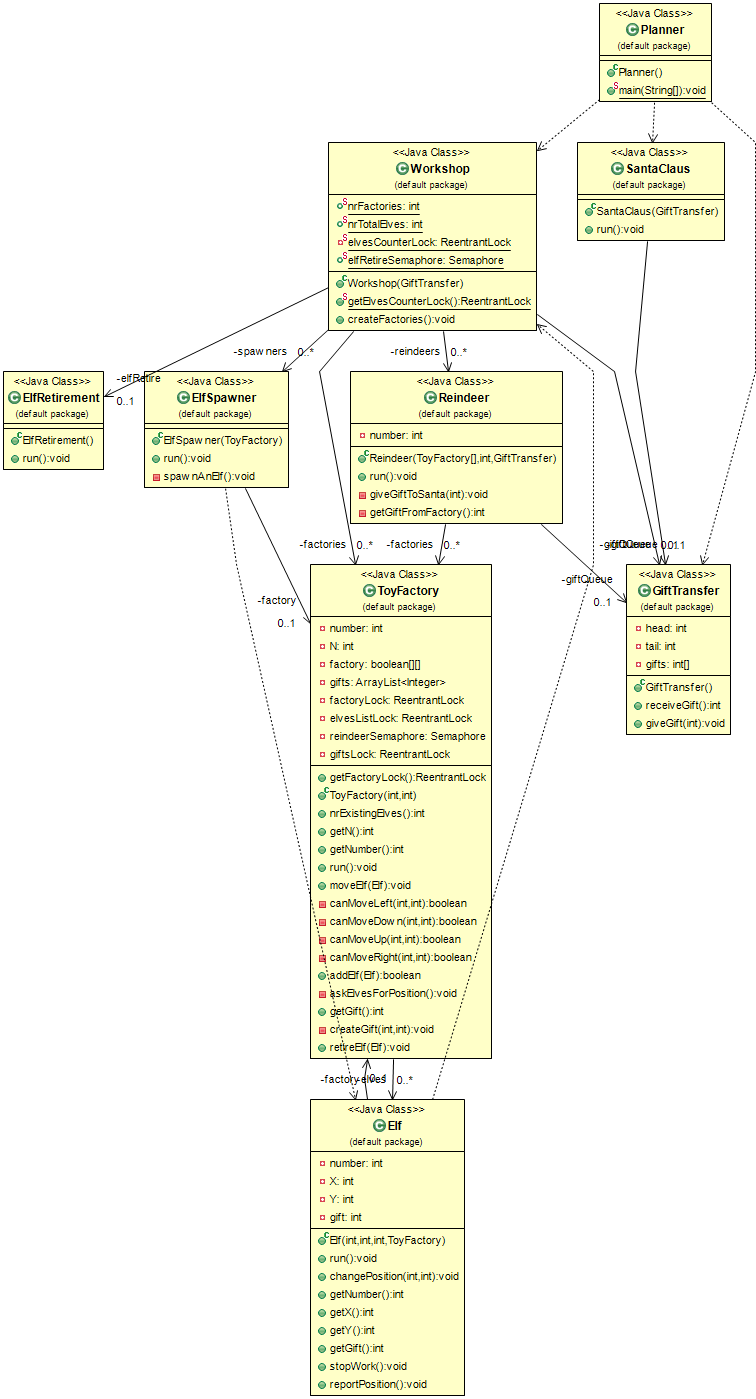
\includegraphics[width=9cm]{UML.png}
\centering
\end{figure}

\section{\textbf{Observations :}}

\begin{itemize}
    \item Since elves are very fast (they only rest 30 milliseconds between creating gifts), reindeers also need to be fast in getting gifts from the factories :
    they will have a sleeping time between 10 and 30 milliseconds.
    \item Multiple reindeers can give gifts to Santa so he must be fast in receiving them (Santa gets no rest between receiving gifts).
    \item If we don't want an elf to immediately retire after creating a gift (moving in the factory), we should give the retirement thread a longer sleeping time between releasing retire permits.
    \item The gift list of a factory can be accessed by only one reindeer at a time, so the reindeer semaphore acts as an access queue to get the gift list lock.
    \item The toy factories will also be working threads since they ask elves to report their positions every 3 seconds.
    \item All factory members that were accessed/modified by multiple parties were synchronized : the matrix, the elves list and the gifts list.
    
\end{itemize}
\vfill
\begin{thebibliography}{9}
\label{sec_ref}

\bibitem{UML}
\url{http://www.objectaid.com/}
 \emph {UML Explorer for Eclipse}.
 
\bibitem{Semaphores}
\url{https://docs.oracle.com/javase/7/docs/api/java/util/concurrent/Semaphore.html}
 \emph {Semaphores in Java}.
 
\bibitem{Locks}
\url{https://docs.oracle.com/javase/7/docs/api/java/util/concurrent/locks/ReentrantLock.html}
 \emph {Locks in Java}.
 
\bibitem{Cyclic Barrier}
\url{https://docs.oracle.com/javase/7/docs/api/java/util/concurrent/CyclicBarrier.html}
 \emph {Cyclic Barrier in Java}.
 
\bibitem{latex}
\LaTeX project site,
\url{http://latex-project.org/}

\end{thebibliography}

 

\vfill
\end{document}



